\documentclass{article}

\usepackage[utf8]{inputenc}
\usepackage{graphicx}
\usepackage{hyperref}
\usepackage{amssymb}
\usepackage{tikz} % add a few drawings ...
\usepackage{tkz-euclide}
\usepackage{tikz-3dplot}
\usetikzlibrary{calc}
\usepackage{pgfplots}
\usepackage{xcolor}

\title{Elements of geodesy}
\date{\today}
\author{Xanthos}

\begin{document}
  
  \maketitle

  %\frontmatter
  \tableofcontents
  \listoffigures
  \listoftables

  % 
  \section{Ellipsoidal Geometry}
  \label{ch:ellipsoidal-geometry}

  \subsection{Latitude Definitions}
  \label{ssec:latitude-definitions}
  
  \textbf{Geodetic latitude} $\phi$, is the angle between the normal (to the 
  ellipsoid) and the equatorial plane.
  \textbf{Geocentric Latitude} $\psi$ (sometimes called \emph{spherical latitude}) is 
  the angle between the radius (from centre to the point on the surface) and 
  the equatorial plane. It is related to \emph{geodetic latitude} by:
  \begin{equation}
    \psi (\phi) = \arctan{\left(\left(1-e^2\right)\tan \phi \right)} 
      = \arctan{\left(\left(1-f\right)^2 \tan \phi \right)}
  \end{equation}
  The \textbf{parametric} or \textbf{reduced} latitude, $u$, is defined 
  by the radius drawn from the centre of the ellipsoid to that point N on the 
  surrounding sphere (of radius $\alpha$) which is the projection parallel to 
  the Earth's axis of a point P on the ellipsoid at latitude $\phi$. The 
  \emph{parametric latitude} is related to the \emph{geodetic latitude} by:
  \begin{equation}
    u(\phi) = \arctan{\left( \sqrt{1-e^2} \tan \phi \right)} 
      = \arctan{\left(\left(1-f\right) \tan \phi \right)}
  \end{equation}
  Note that in astronomy, $u$ is oftenly called \textbf{eccentric anomaly} 
  (normally denoted as $E$).

  \begin{figure}
    \centering
      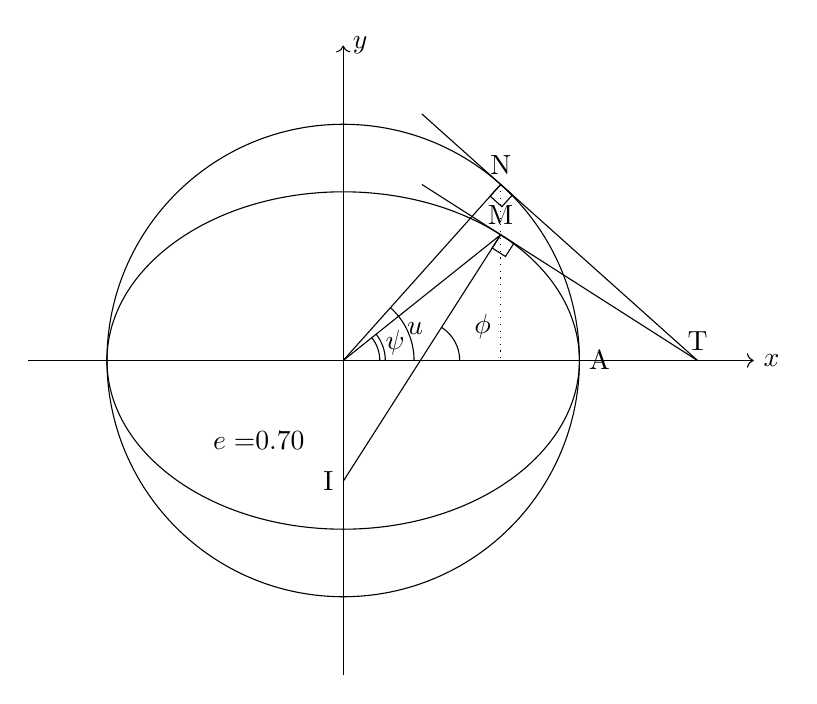
\begin{tikzpicture}

  \pgfmathsetmacro{\semimajor}{+3.0000000000};
  \pgfmathsetmacro{\semiminor}{+2.1424285286};
  \pgfmathsetmacro{\eccentricity}{0.70};
  \coordinate (N)  at (+2.0000000000, +2.2360679775);
  \coordinate (M)  at (+2.0000000000, +1.5968719423);
  \coordinate (T)  at (+4.5000000000, +0.0000000000);
  \coordinate (TC) at (+1.0000000000, +3.1304951685);
  \coordinate (TE) at (+1.0000000000, +2.2356207192);
  \coordinate (XEND) at (+5.2141428429, +0.0000000000);
  \coordinate (I) at (+0.0000000000, -1.5342495132);
  \coordinate (II) at (+0.9800000000, +0.0000000000);
  \coordinate (TXT) at (-1.0712142643, -1.0228330088);
  \coordinate (MP) at (+2.0000000000, +0.0000000000);

  \node (t) at (T) [above]{T};
  \node (m) at (M) [above]{M};
  \node (n) at (N) [above]{N};
  \node (a) at (\semimajor,0) [below, right]{A};
  \node (i) at (I) [left]{I};
  %\node (tc) at (TC) {TC};
  %\node (te) at (TE) {TE};
  \node (txt) at (TXT) {$e=$\eccentricity};
  \coordinate (O) at (0e0,0e0);
  
  \draw (0,0) ellipse (\semimajor cm and \semiminor cm);
  \draw (0,0) circle (\semimajor);
  
  \draw[->] ($(-\semimajor -1 , 0)$)--(XEND) node[right]{$x$};
  \draw[->] ($(0, -\semimajor -1)$)--($(0, \semimajor +1)$) node[right]{$y$};

  \draw (TC) -- (T);
  \draw (TE) -- (T);
  \draw (N) -- (O);
  \draw (M) -- (O);
  \draw (M) -- (I);
  \draw[dotted] (N) -- (M) -- (MP);

  \tkzMarkRightAngle[draw=black,size=.2](T,N,O);
  \tkzMarkRightAngle[draw=black,size=.2](T,M,I);
  \tkzMarkAngle[size = .5, arc=ll](T,O,M)
  \tkzLabelAngle[pos=.7](T,O,M){$\psi$};
  \tkzMarkAngle[size = .9, arc=l](T,O,N)
  \tkzLabelAngle[pos=1.0](T,O,N){$u$};
  \tkzMarkAngle[size = .5, arc=l](T,II,M)
  \tkzLabelAngle[pos=.9](T,II,M){$\phi$};

\end{tikzpicture}

      \caption{Different latitude definitions.}
      \label{fig:latitude-definitions}
  \end{figure}
  \begin{table}[h!]
    \centering
    \begin{tabular}{| c | c | c | c|}
      \hline
      \textbf{Latitude} & \textbf{Symbol} & \textbf{Reference Direction} & \textbf{Angle} \\
      \hline
      geocentric & $\psi$ & centre of the Earth & $\angle{AOM}$ \\
      geodetic   & $\phi$ & normal to the ellipsoid & $\angle{OA,IM}$ \\
      parametric & $u$    & centre of the Earth & $\angle{AON}$ \\
      \hline
    \end{tabular}
    \caption{Latitude definitions, see \ref{fig:latitude-definitions}.}
    \label{table:latitude-definitions}
\end{table}
  
  \subsection{Coordinates Types}
  \label{ssec:coordinates-types}
  \textbf{Geodetic coordinates} $(\lambda, \phi, h)$ are a type of curvilinear 
  orthogonal coordinate system based on a reference ellipsoid. They include the 
  \emph{geodetic latitude} $\phi$, the \emph{longitude} $\lambda$ and the 
  \emph{ellipsoidal height} $h$ (also known as \emph{geodetic height}). Geodetic 
  coordinates are also commonly known as \textbf{Earth ellipsoidal coordinates}. 
  By convention, $\lambda \in \left[-\pi, \pi \right]$ and 
  $\phi \in \left[-\pi/2, \pi/2 \right]$.

  \textbf{Spherical coordinates} are defined by the triad \emph{radial distance} 
  $r$, \emph{polar distance} $\theta$ and \emph{geocentric longitude} $\lambda$ 
  The polar angle may be called \emph{colatitude, zenith angle, normal angle}, or 
  \emph{inclination angle}. It is often denoted as $\phi$, but here we will adopt 
  the $\theta$. \emph{geocentric longitude} $\lambda$ is often also called \emph{azimouthal angle} 
  and denoted by $\theta$.
  \begin{figure}
    \centering
      \pgfplotsset{compat=1.6}
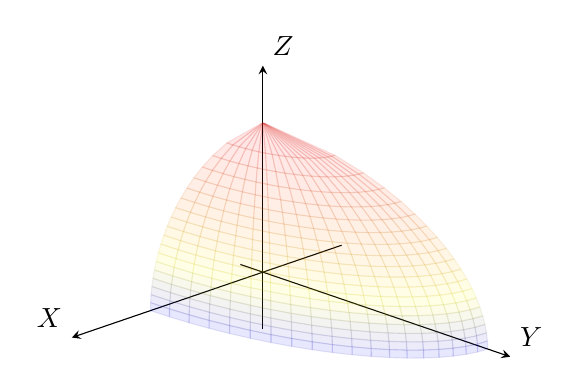
\begin{tikzpicture}
\begin{axis}
  [view={135}{20},
    axis lines=center, axis on top,ticks=none,
    set layers=default,axis equal,
    xlabel={$X$}, ylabel={$Y$}, zlabel={$Z$},
    xlabel style={anchor=south east},
    ylabel style={anchor=south west},
    zlabel style={anchor=south west},
    enlargelimits,
    tick align=inside,
    domain=0:2.00,
    samples=20, 
    z buffer=sort,
  ]
  \addplot3 [surf,opacity=0.1,domain=0:1,
    domain y=0:90,on layer=axis foreground] ({sin(y)*sqrt(1-x^2)},{2*cos(y)*sqrt(1-x^2)},{x});
\end{axis}
\end{tikzpicture}

%\tdplotsetmaincoords{80}{120}
%%
%\pgfmathsetmacro{\rvec}{1.2}
%\pgfmathsetmacro{\thetavec}{40}
%\pgfmathsetmacro{\phivec}{60}
%\pgfmathsetmacro{\smajor}{1}
%\pgfmathsetmacro{\sminor}{1}
%%
%\begin{tikzpicture}[scale=5,tdplot_main_coords]
%  \coordinate (O) at (0,0,0);
%  \draw[thick,->] (0,0,0) -- (1,0,0) node[anchor=north east]{$x$};
%  \draw[thick,->] (0,0,0) -- (0,1,0) node[anchor=north west]{$y$};
%  \draw[thick,->] (0,0,0) -- (0,0,1) node[anchor=south]{$z$};
%  
%  \tdplotsetcoord{P}{\rvec}{\thetavec}{\phivec}
%  \draw[-stealth,color=black] (O) -- (P);
%  \draw[dashed, color=black] (O) -- (Pxy);
%  \draw[dashed, color=black] (P) -- (Pxy);
%  \tdplotdrawarc{(O)}{0.2}{0}{\phivec}{anchor=north}{$\lambda$}
%  
%  %\tdplotsetthetaplanecoords{\phivec}
%  %\tdplotdrawarc[tdplot_rotated_coords]{(0,0,0)}{0.5}{0}%
%  %{\thetavec}{anchor=south west}{$\theta$}
%  %\draw[dashed,tdplot_rotated_coords] (\rvec,0,0) arc (0:90:\rvec);
%  %\draw[dashed] (\rvec,0,0) arc (0:90:\rvec);
%  %\tdplotsetrotatedcoords{\phivec}{\thetavec}{0}
%  %\tdplotsetrotatedcoordsorigin{(P)}
%  %\draw[thick,tdplot_rotated_coords,->] (0,0,0) -- (.5,0,0) node[anchor=north west]{$x’$};
%  %\draw[thick,tdplot_rotated_coords,->] (0,0,0) -- (0,.5,0) node[anchor=west]{$y’$};
%  %\draw[thick,tdplot_rotated_coords,->] (0,0,0) -- (0,0,.5) node[anchor=south]{$z’$};
%  %\draw[-stealth,color=blue,tdplot_rotated_coords] (0,0,0) -- (.2,.2,.2);
%  %\draw[dashed,color=blue,tdplot_rotated_coords] (0,0,0) -- (.2,.2,0);
%  %\draw[dashed,color=blue,tdplot_rotated_coords] (.2,.2,0) -- (.2,.2,.2);
%  %\tdplotdrawarc[tdplot_rotated_coords,color=blue]{(0,0,0)}{0.2}{0}%
%  %{45}{anchor=north west,color=black}{$\phi’$}
%  %\tdplotsetrotatedthetaplanecoords{45}
%  %\tdplotdrawarc[tdplot_rotated_coords,color=blue]{(0,0,0)}{0.2}{0}%
%  %{55}{anchor=south west,color=black}{$\theta’$}
%\end{tikzpicture}

      \caption{Topocentric coordinates.}
      \label{fig:topocentric-crd}
  \end{figure}

\end{document}
